%
% Solutions (Handouts) to the exercises
%

\chapter{Solutions to exercises}

\section{Solutions for Chapter 1}

\begin{Solution}{Photoabsorption}
\textbf{Photoabsorption}\\
\end{Solution}

\begin{Solution}{Monte-Carlo_Integration}
  \textbf{Monte-Carlo Integration -- Speed and Accuracy -- \texttt{photoabsorption.m}}\\
  \begin{enumerate}
  \item Hit and Miss Method -- \texttt{hitandmiss.m, hitandmiss2.m} \\
    The estimate for the integral is $I_i=n_i/n$, where $n_i$ are the
    number of hits in one realization. By doing $N$ realizations of
    the method, you estimate the integral by using the mean of the
    generated $I_i, i=1,\ldots,N$. The mean is estimated by the
    well known formula
    $$ \overline{I}=\frac{1}{N} \sum_{i=1}^N I_i .$$
    (Use the function \texttt{mean()} from Matlab.)
    The error of the individual trial $I_i$ gets estimated by using
    the standard deviation. We estimate the standard deviation $\sigma_i$
    by using
    $$ \sigma_{I_i} = \frac{1}{N-1} \sum_{i=1}^N \left( I_i - \overline{I}
       \right)^2 .$$
    (We can use the Matlab function \texttt{std()} for calculating the
    standard deviation.)
    This is the error of the individual trial $I_i$, not the error of the
    mean value $\overline{I}$ calculated above. To that end, we have to
    use the central limit theorem and get
    $$ \sigma_{\overline{I}} = \sigma_{I_i} / \sqrt{N} .$$

    Some example outputs of the program: \\[0.5cm]
    left: One realization using up to 5000 points in steps of 50. \\
    right: Up to 10000 realizations using stepsize 100 and 50 points for
      each realization. \\
      \begin{center}
        \hspace*{-1cm}
        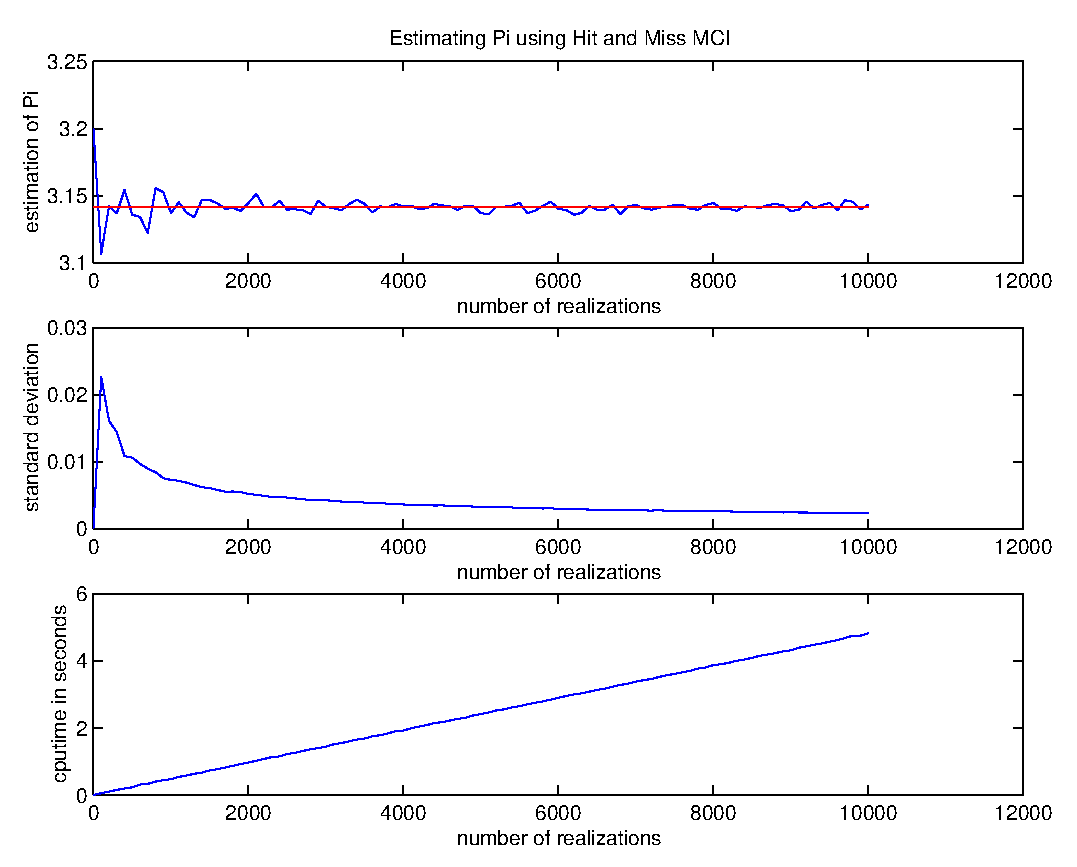
\includegraphics[width=0.44\textwidth]{f_Hit_and_Miss2_1.eps} \hfill
        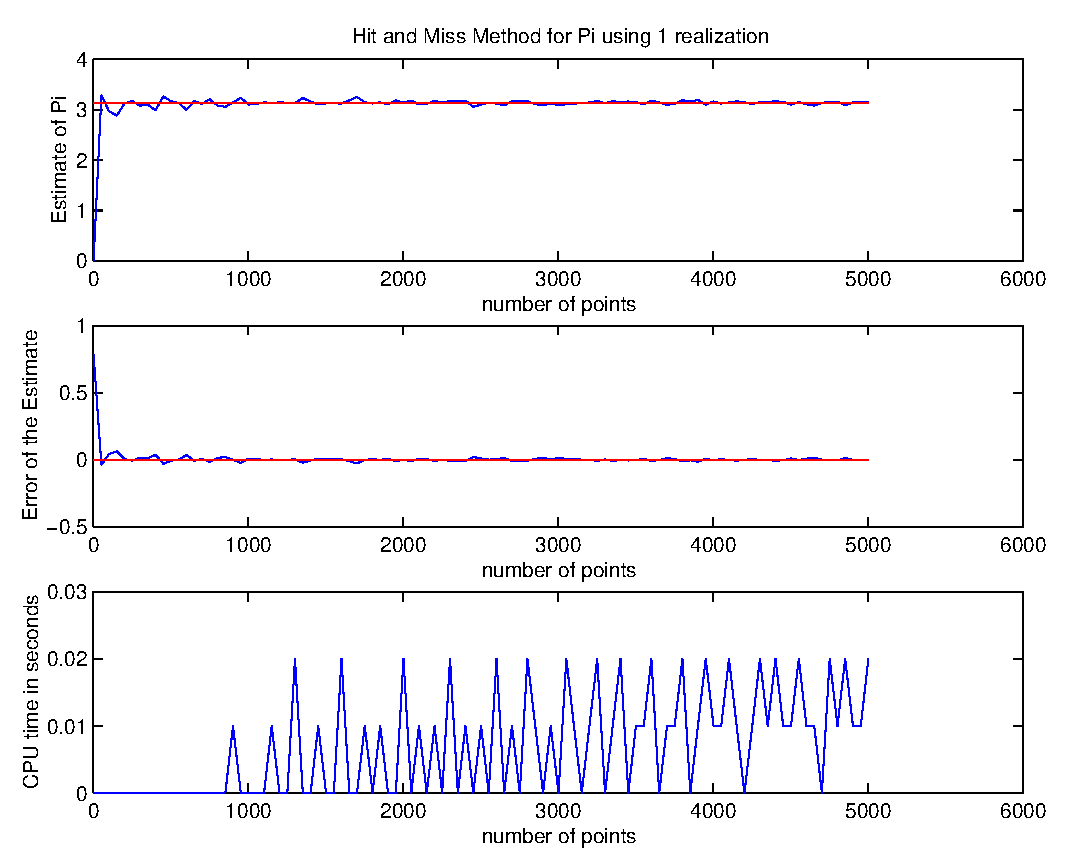
\includegraphics[width=0.44\textwidth]{f_Hit_and_Miss2_2.eps}
      \end{center}

  \item Standard Method -- \texttt{mcistandard.m}\\
    Now we use the formula $I_i=\frac{1}{n} \sum_{i=1}^n f(x_i) (b-a) $
    to estimate the integral. The mean value is
    $$ \overline{I}_i =\frac{1}{n} \sum_{i=1}^n I_i ,$$
    and the standard deviation of the individual $I_i$ is
    $$ \sigma_{I_i} = \frac{1}{N-1} \sum_{i=1}^N \left( I_i - \overline{I}
       \right)^2 = \sigma_{\overline{I}_i} \times \sqrt{n} ,$$
    where we have used the central limit theorem for the last equation to
    get the error of the mean $\sigma_{\overline{I}_i}.$

    Now we calculate several ($N$) realizations of the above algorithm
    to get a better estimate of the integral. The mean of the ensemble
    of realizations is
    $$ \overline{I}_N = \frac{1}{N} \sum_{i=1}^N \overline{I}_i . $$
    And the error of the mean is
    $$ \sigma_{\overline{I}_N} = \frac{1}{N-1} \sum_{i=1}^N \left(
      \overline{I}_i - \overline{I}_N \right)^2 =
      \sigma_{\overline{I}_i} / \sqrt{N} . $$
    Again we have used the central limit theorem and assumed that
    we have a ``representative'' $\sigma_{\overline{I}_i}$ to get
    the last equality.

    Some example outputs of the program: \\[0.5cm]
    left: Using increasing ensemble size from 1 to 5000 in steps of 100.
          Always using 50 points in the interval (a,b).\\
    right: The standard deviation and the distance to the exact result
           for the same run as in the left figure.\\
      \begin{center}
        \hspace*{-1cm}
        \includegraphics[width=0.44\textwidth]{f_MCI_Standard_3.eps} \hfill
        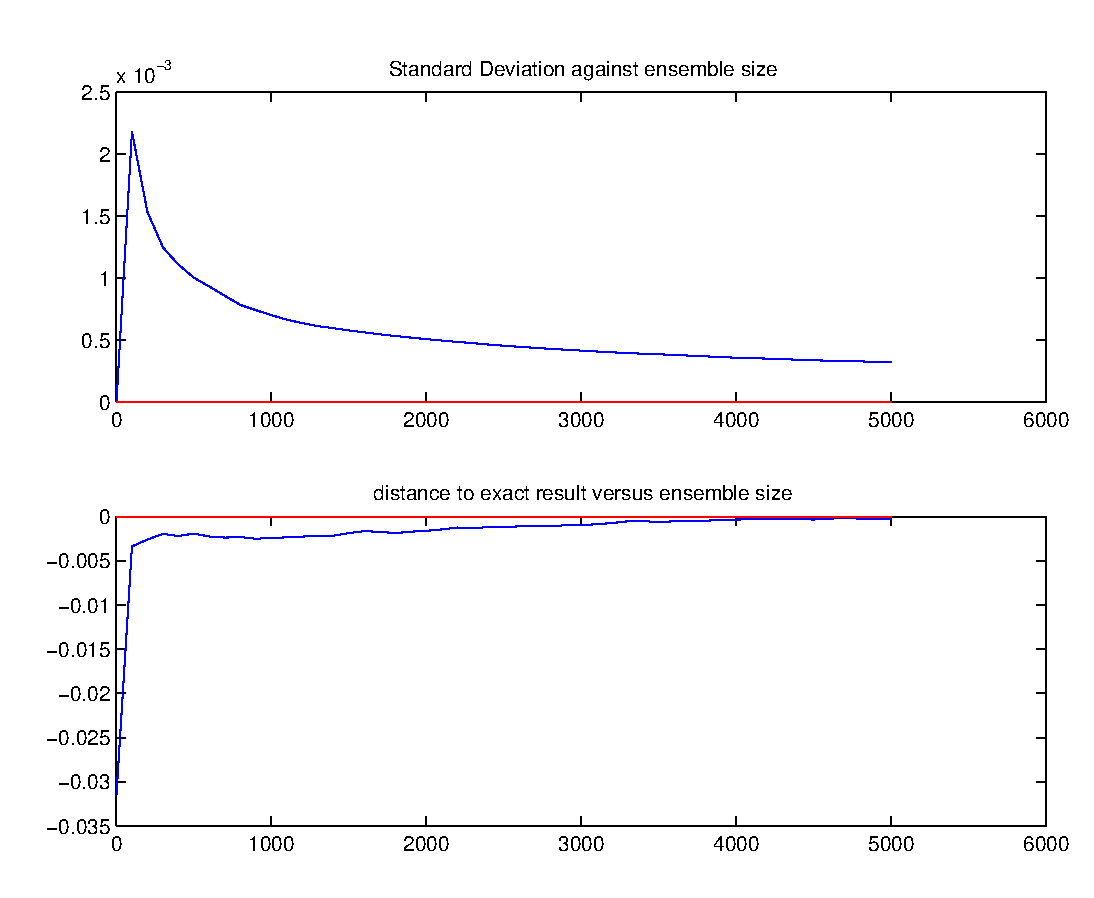
\includegraphics[width=0.44\textwidth]{f_MCI_Standard_2.eps}
      \end{center}
    The CPU time used plotted versus the accurracy of the estimate.
      \begin{center}
        \hspace*{-0.5cm}
        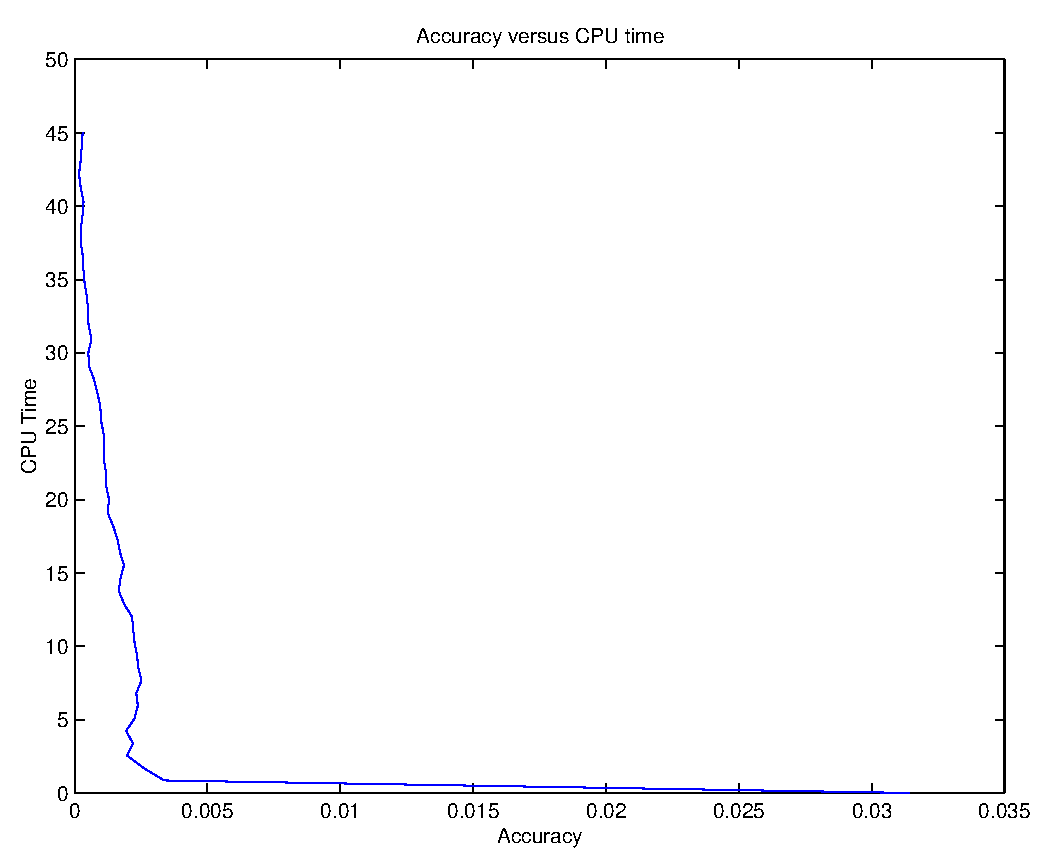
\includegraphics[width=0.5\textwidth]{f_MCI_Standard_1.eps}
      \end{center}

   \end{enumerate}
\end{Solution}

\begin{Solution}{Euler_Constant}
\textbf{Euler��s Constant using Monte-Carlo Algorithm -- \texttt{darts.m}} \\
\end{Solution}

%%%%%%%%%%%%%%%%%%%%%%%%%%%%%%%%%%%%%%%%%%%%%%%%%%%%%%%%%%%%%%%
\section{Solutions to Chapter 2}

\begin{Solution}{Random-Number_Generator_Check}
\textbf{Random-Number Generator Check - \texttt{momentsrand.m, pokertest.m}} \\
  \begin{itemize}
  \item Moments of the \texttt{rand()} function of Matlab\\
    Example output for the first 10 moments of \texttt{rand()} using
    5000 random numbers. Shown are the mean moments of the ensemble,
    the error (standard deviation) of the mean and in the last plot
    the distribution as a histogram using 50 bins.
   \begin{center}
      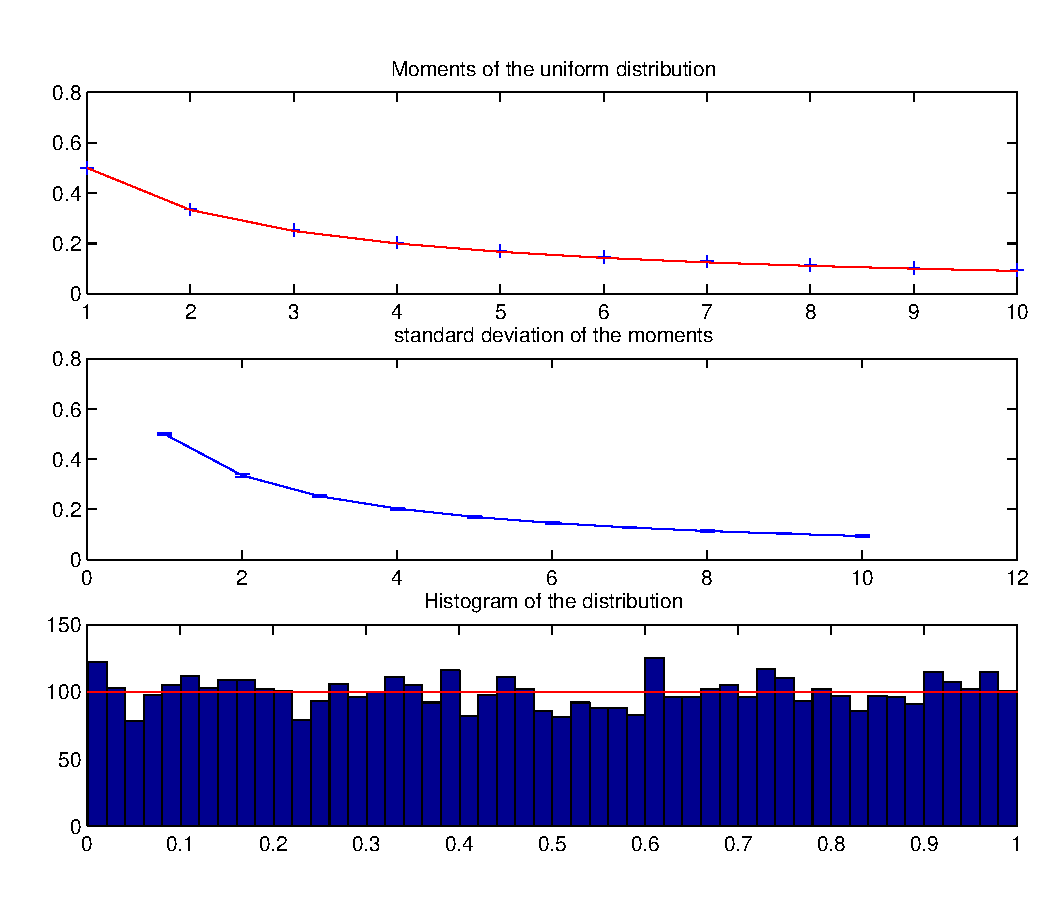
\includegraphics[width=0.8\textwidth]{f_Moments_Rand.eps}
    \end{center}
  \item Poker Test \\
    Shown are the results for a Poker test using 20000 hands, each
    using 5 random numbers (=cards). Only no pairs (=0), pairs (=1),
    three of a kind (=3) and four of a kind (=4) are counted (5 of
    a kind is obviously not allowed). The numbers above the bars are
    the actual number of hands found in the ensemble. The second plot
    shows the difference of the probability in our ensemble to the
    correct theoretical result.
    \begin{center}
      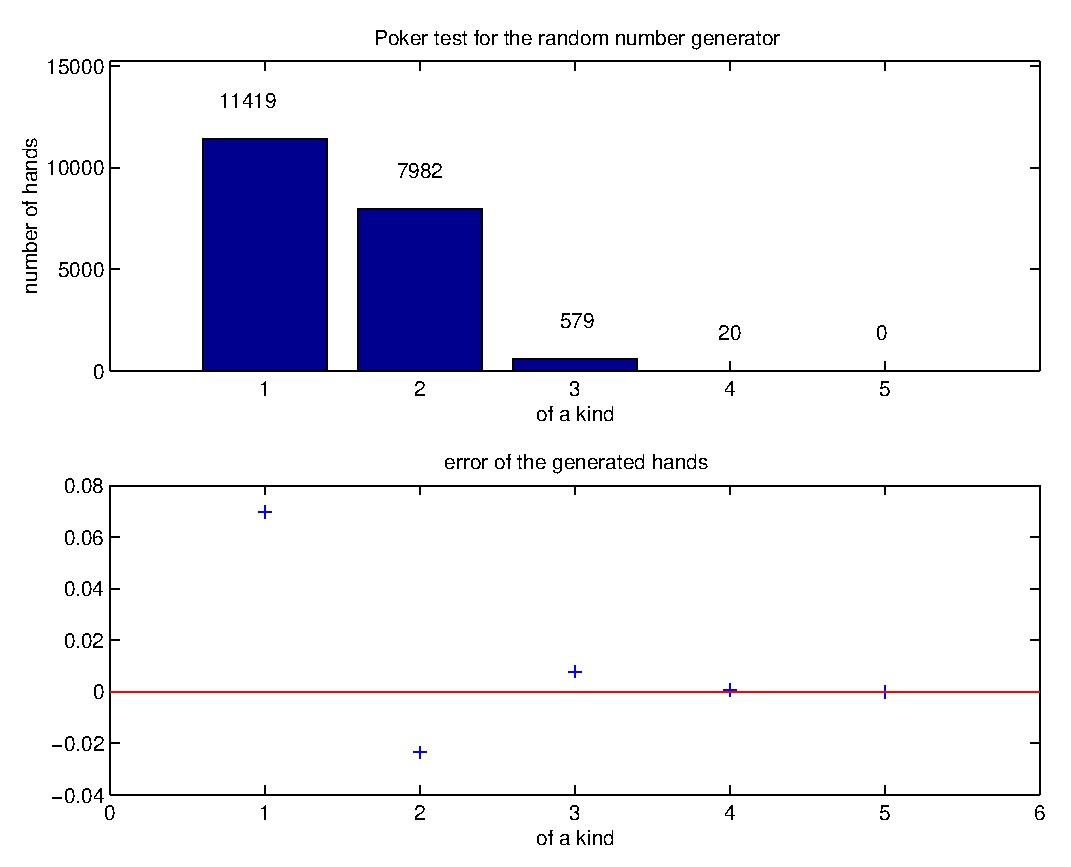
\includegraphics[width=0.8\textwidth]{f_Poker_Test.eps}
   \end{center}
 \end{itemize}   
\end{Solution}

\begin{Solution}{Galton_Board}
\textbf{Galton Board and Pascal Triangle  - \texttt{galton\_board.m}} \\
  Examples of the Galton Boards. We plot the boxes at the lower end of
  the Galton board versus the number of balls, which have fallen into
  each box. The red line indicates the normal distribution with the
  same variance and the maximum height as the ensemble generated.\\[0.5cm]
  left: using 10 rows of pins and 1000 balls \\
  right: using 20 rows of pins and 1000 balls
    \begin{center}
      \hspace*{-1cm}
      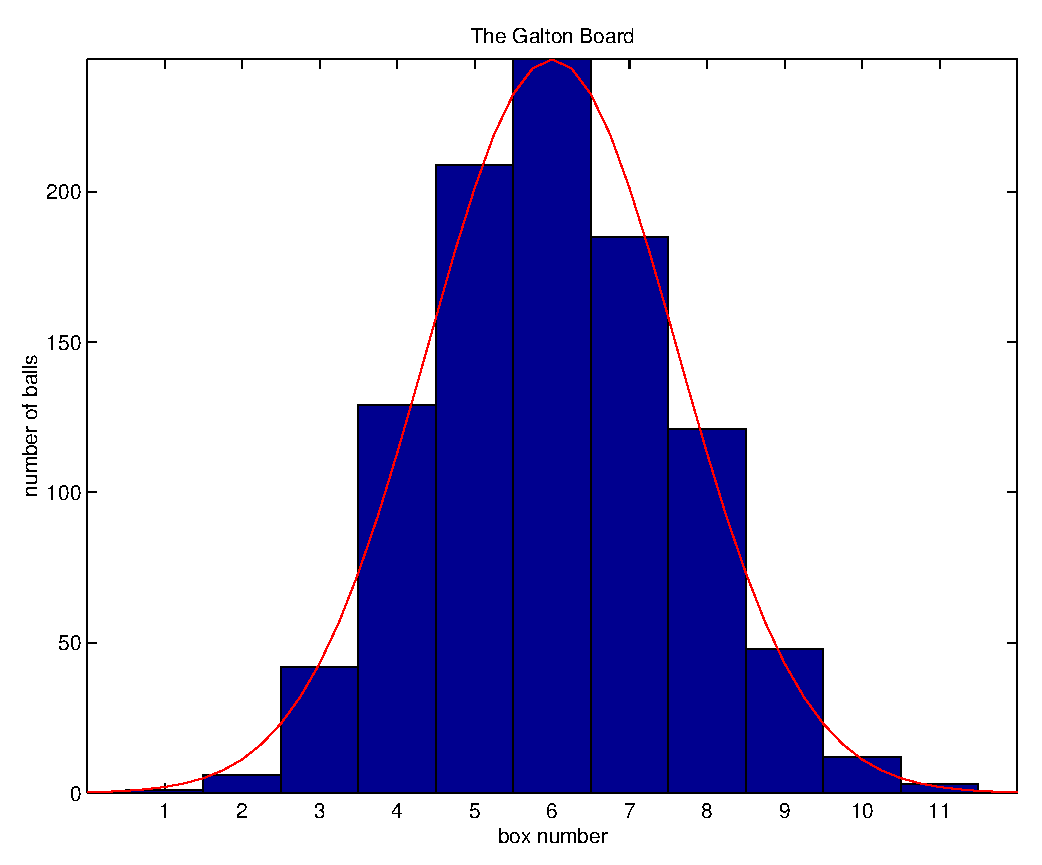
\includegraphics[width=0.45\textwidth]{f_Galton_board_3.eps}\hfill
      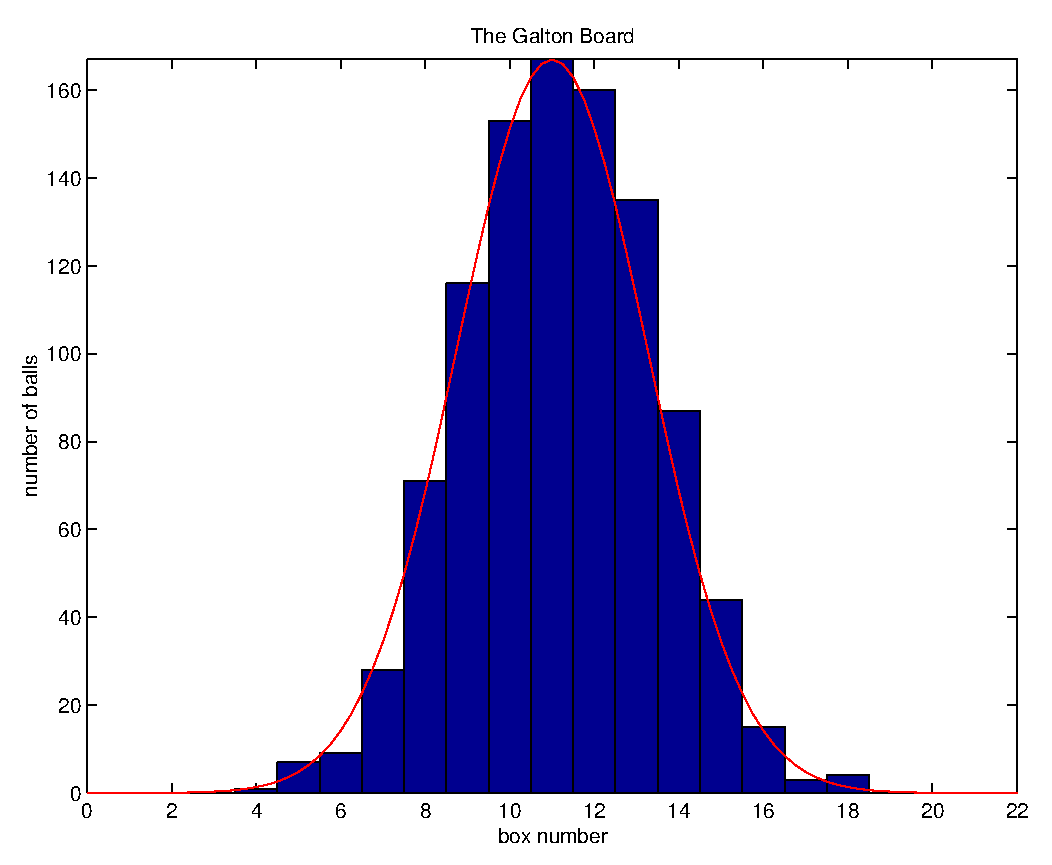
\includegraphics[width=0.45\textwidth]{f_Galton_board_1.eps}
   \end{center}

   \newpage
   using 200 rows and 16000 balls
    \begin{center}
      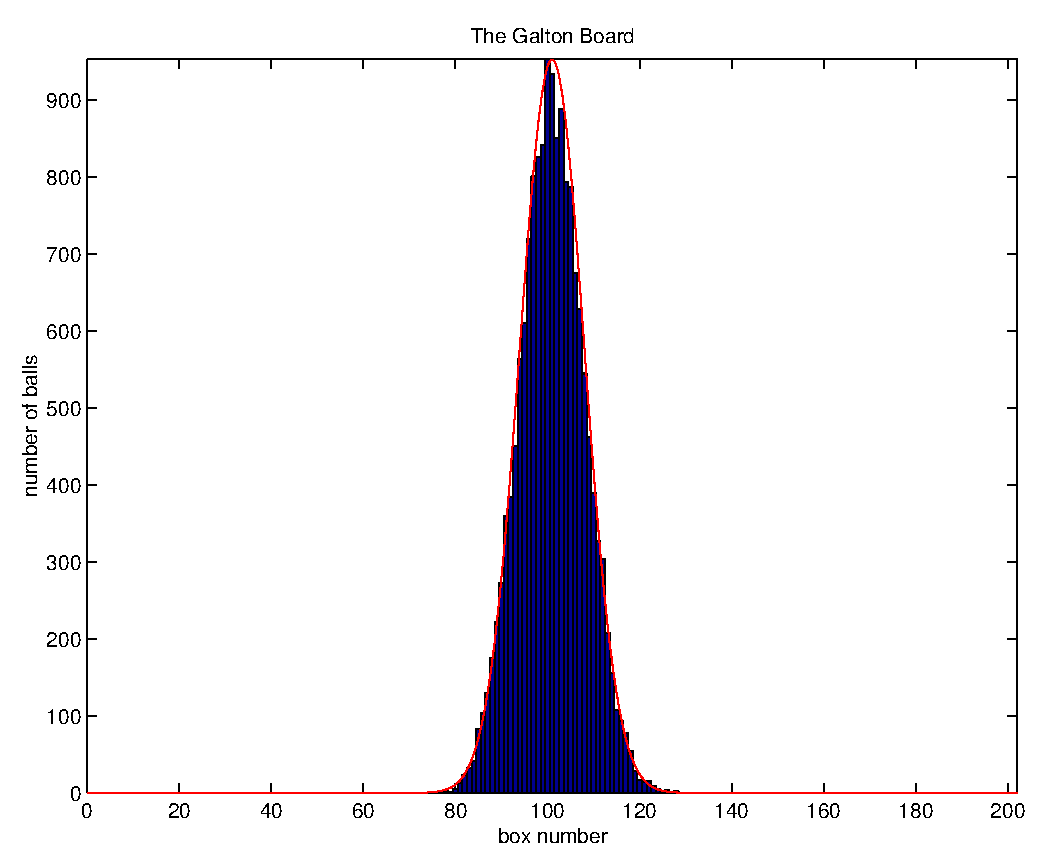
\includegraphics[width=0.8\textwidth]{f_Galton_board_2.eps}
   \end{center}

   The connection to the Pascal trinagle is obvious, if you know how to
   get the number of balls in the next row (say n+1) from the number of
   balls in the boxes of the previous row (say n). That��s exactly like
   in the Pascal triangle:
   \begin{center}
     1 \\
     1 1 \\
     1 2 1 \\
     1 3 3 1 \\
     1 4 6 4 1 \\
     1 5 10 10 5 1 \\
     1 6 15 20 15 6 1
   \end{center}
   You start with row 2 of the Pascal triangle, which corresponds to
   one pin (1 row) in the Galton board. The sum in each row is $2^N$ in
   row $N$. Therefore the probability for each box of a row of the
   Galton board is just the corresponding number of the Pascal triangle
   divided by $2^N.$          
\end{Solution}

%%%%%%%%%%%%%%%%%%%%%%%%%%%%%%%%%%%%%%%%%%%%%%%%%%%%%%%%%%%%%%%
\section{Solutions to Chapter 3}

\begin{Solution}{Random-Number_Generator}
\textbf{Random-Number Generator - \texttt{linear\_con.m} } \\
    All plots use the linear congruential method with the parameters
    given in the assignment. The input parameters are: Initial seed $1$
    and 1000 random numbers are generated.

    The first plots show the generated random numbers, the second ones
    show the histogram of the distribution. The third ones show 2D vectors
    and the fourth ones 3D vectors from the generated sequence of random
    numbers.
    \begin{itemize}
    \item parameter set 1 \\
      \begin{center}
        \hspace*{-1cm}
        \includegraphics[width=0.47\textwidth]{f_linear_con1a.eps}\hfill
        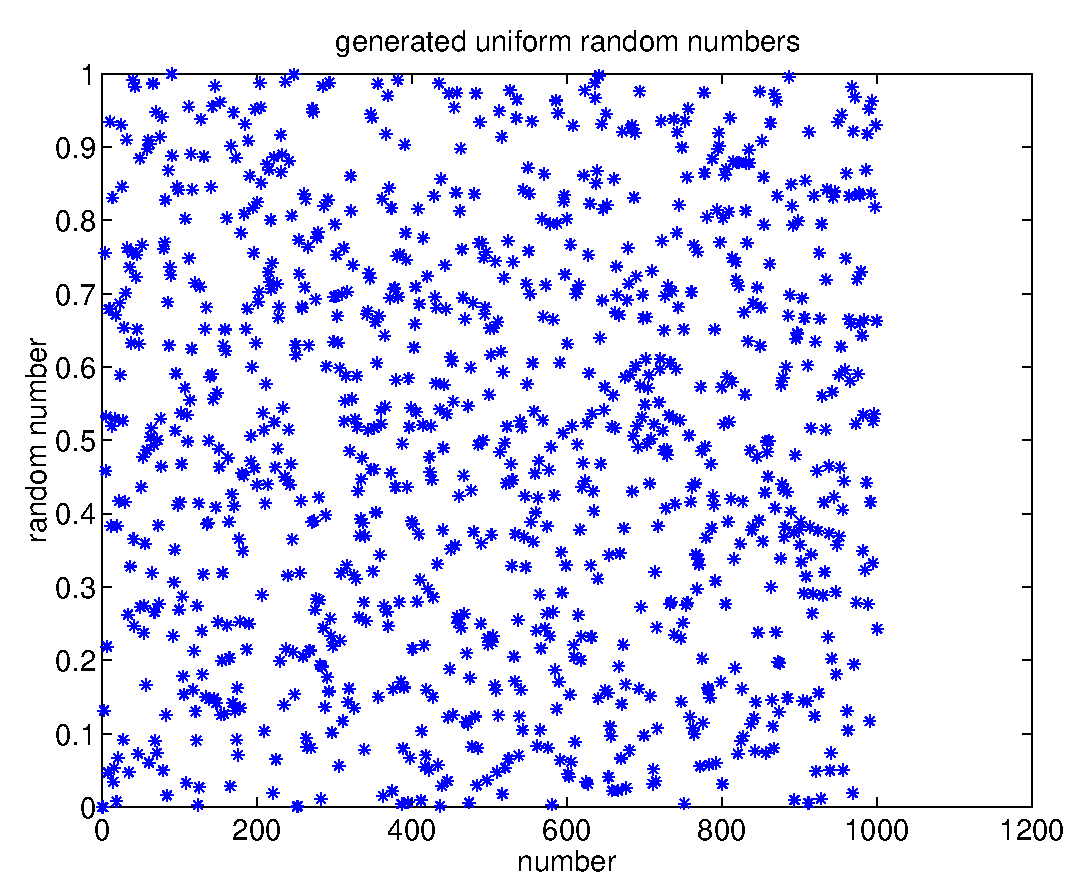
\includegraphics[width=0.47\textwidth]{f_linear_con1b.eps}
      \end{center}
      \begin{center}
        \hspace*{-1cm}
        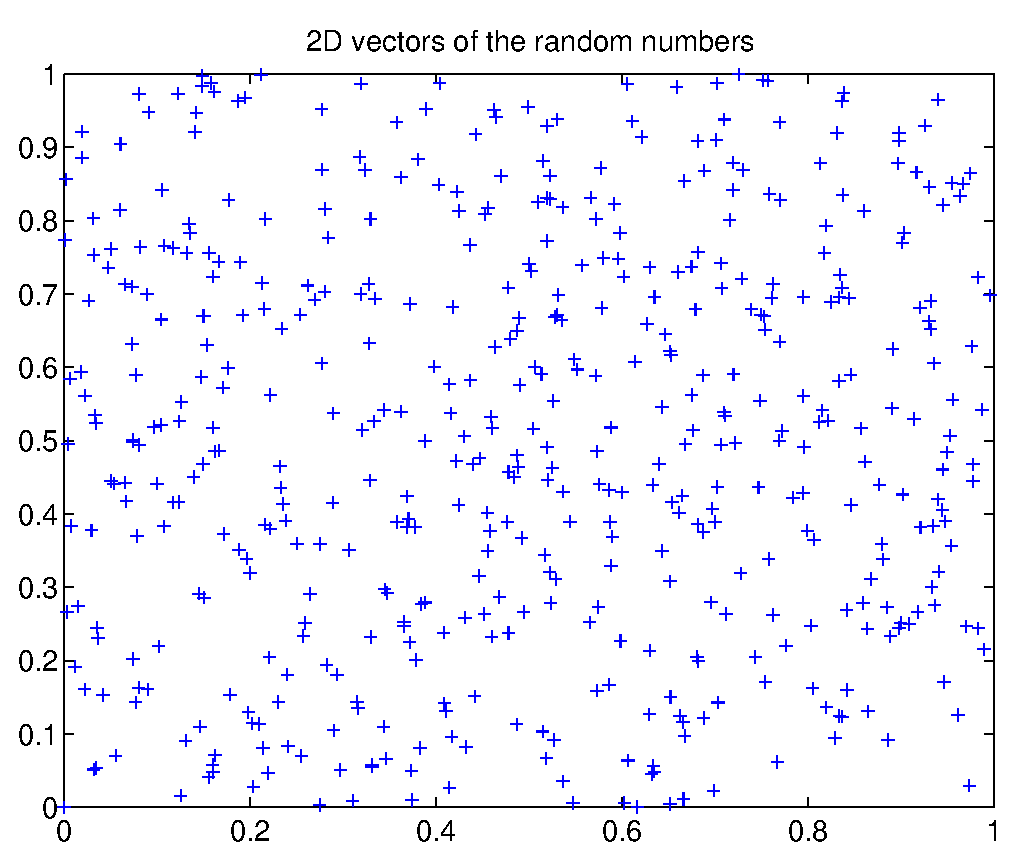
\includegraphics[width=0.47\textwidth]{f_linear_con1c.eps}\hfill
        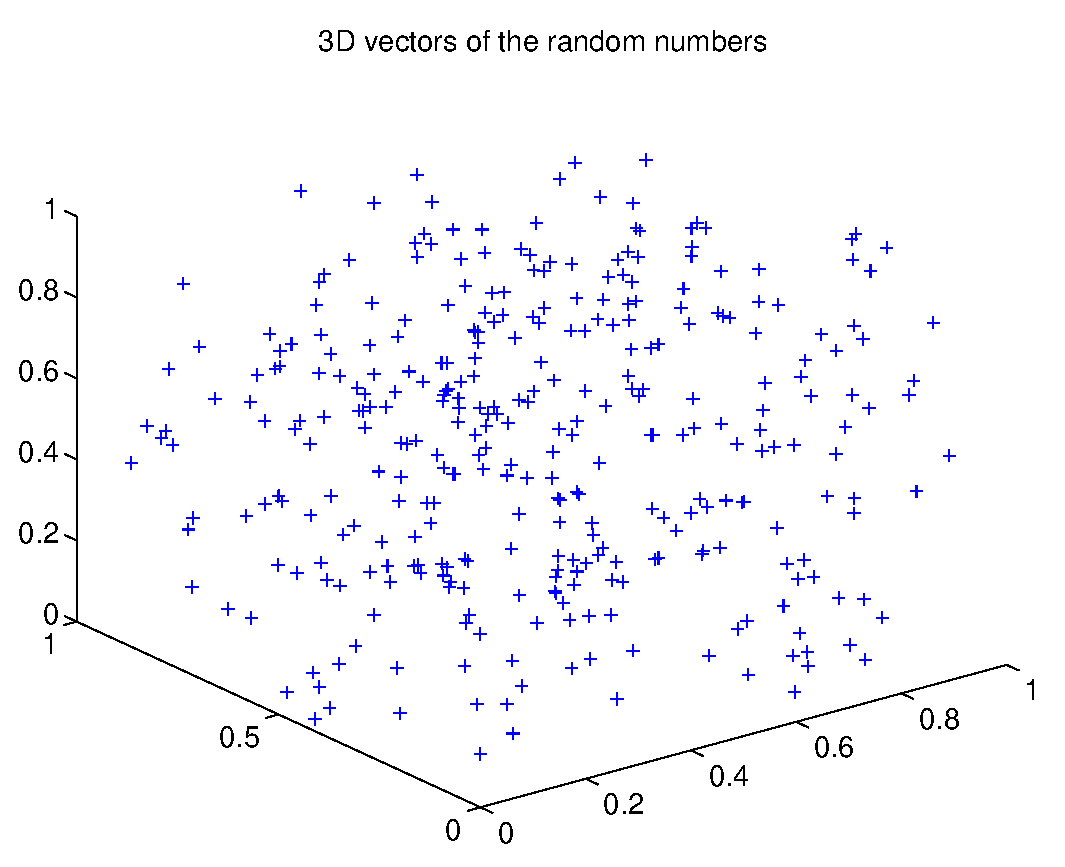
\includegraphics[width=0.47\textwidth]{f_linear_con1d.eps}
      \end{center}
    \newpage
    \item parameter set 2 \\
      \begin{center}
        \hspace*{-1cm}
        \includegraphics[width=0.47\textwidth]{f_linear_con2a.eps}\hfill
        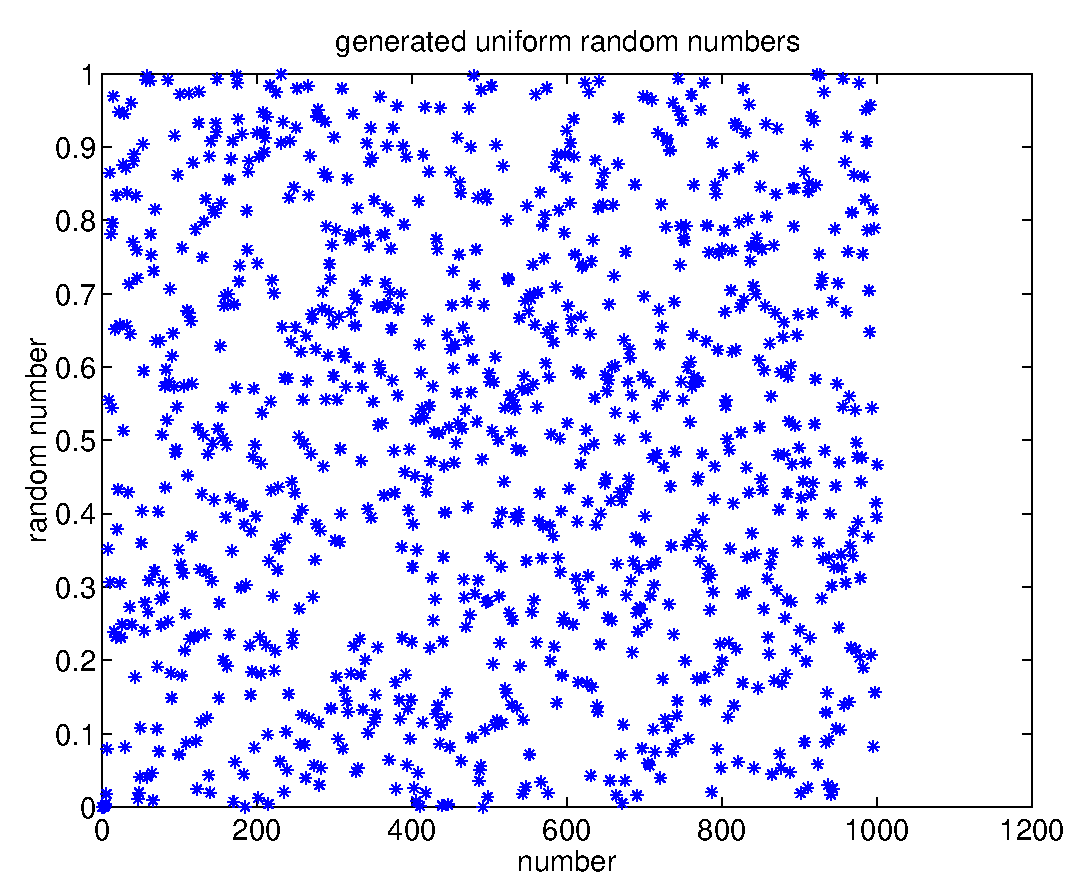
\includegraphics[width=0.47\textwidth]{f_linear_con2b.eps}
      \end{center}
      \begin{center}
        \hspace*{-1cm}
        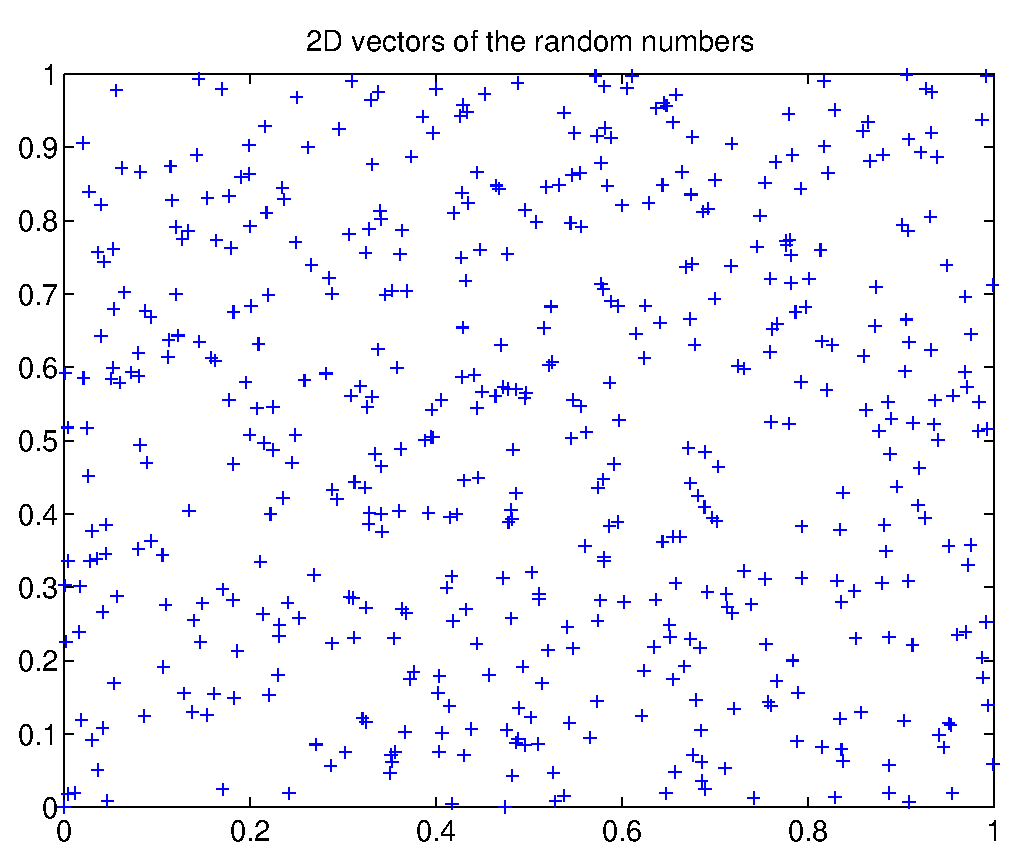
\includegraphics[width=0.47\textwidth]{f_linear_con2c.eps}\hfill
        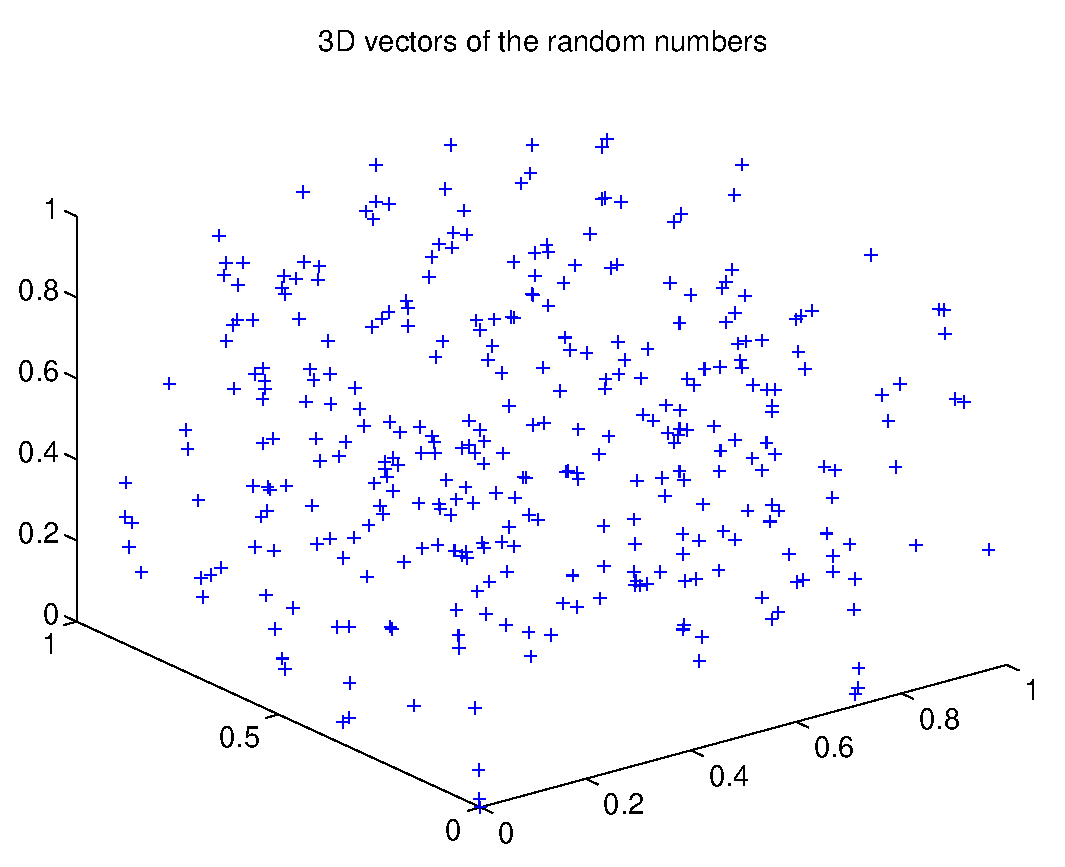
\includegraphics[width=0.47\textwidth]{f_linear_con2d.eps}
      \end{center}
    \end{itemize} 

    At first you don��t see any difference between the two and you
    don��t think of any problems. But if you plot the 3D vectors and
    use the \texttt{rotate3d} command with Matlab to rotate the
    3D plot, you can see plots like the ones below. On the left the
    plot is rotated until you see the planes and on the right you wouldn��t
    expect correlations. Both plots use the same sample of 5000 random numbers.
    This clearly
    visualizes the correlation between successive triple random numbers.
    \begin{center}
      \hspace*{-1cm}
      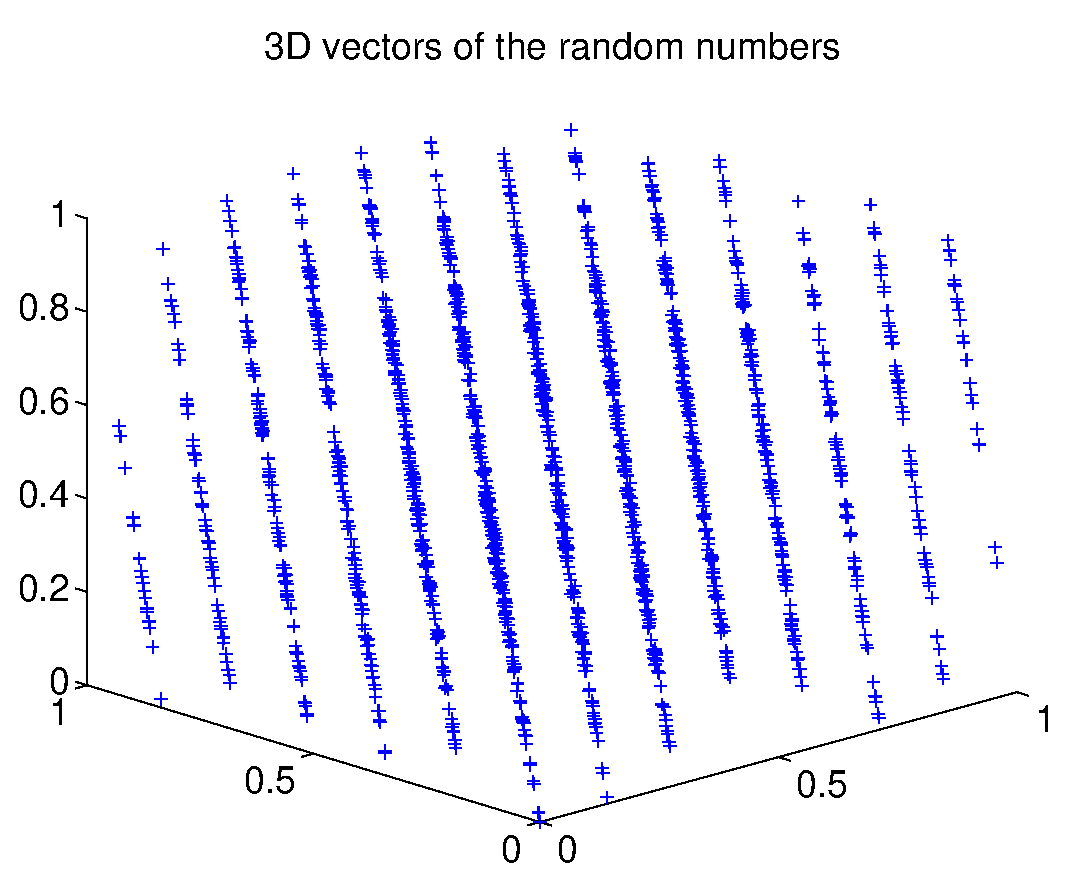
\includegraphics[width=0.47\textwidth]{f_linear_con_3d_1.eps}\hfill
      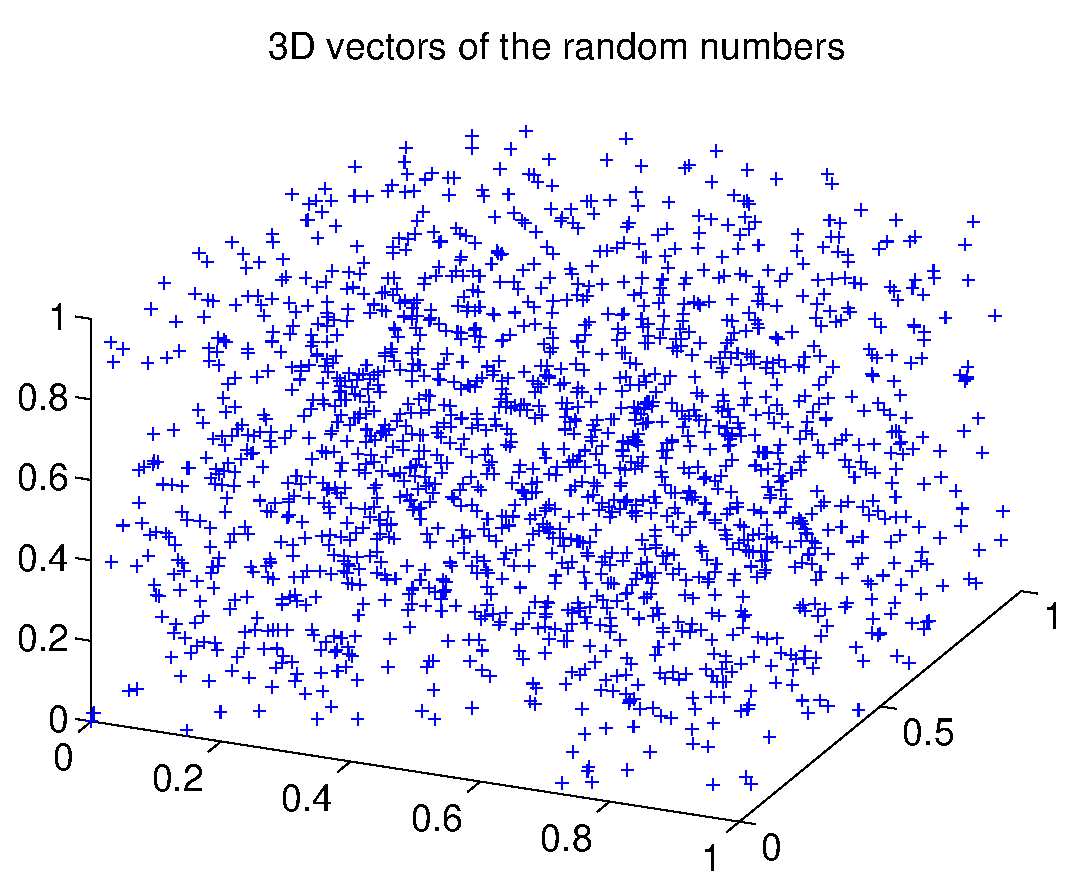
\includegraphics[width=0.47\textwidth]{f_linear_con_3d_2.eps}
    \end{center}
\end{Solution}

\begin{Solution}{Poisson_Distribution}
\textbf{Poisson distribution - \texttt{poisson.m}} \\
  The first figure shows the generated Poisson distributed random
  numbers. The second figure shows two dimensional vectors of Poisson
  distributed random numbers. The last (third) figure finally shows
  the histogram of the generated sequence and the exact Poisson
  distribution.

  The parameters for this run have been:
  $$\lambda = 10 \quad \text{and}\quad N=1000 \quad .$$

  \begin{center}
    \hspace*{-1cm}
    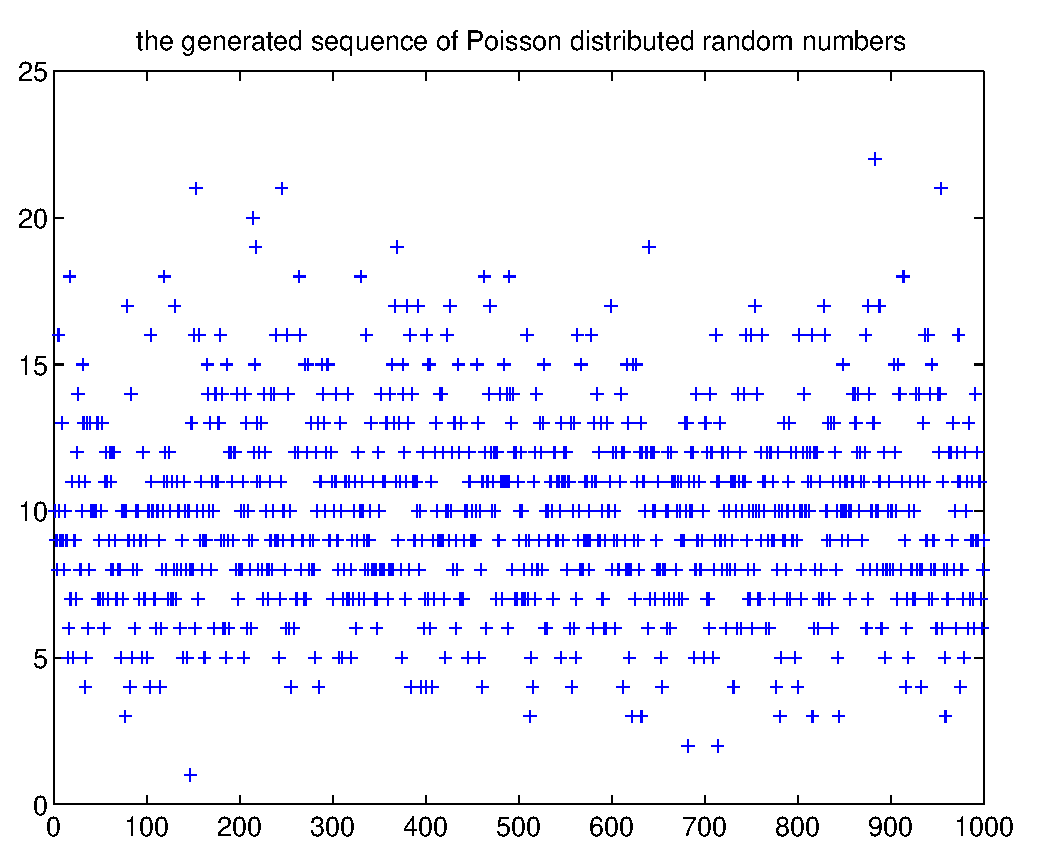
\includegraphics[width=0.47\textwidth]{f_poisson_1.eps}\hfill
    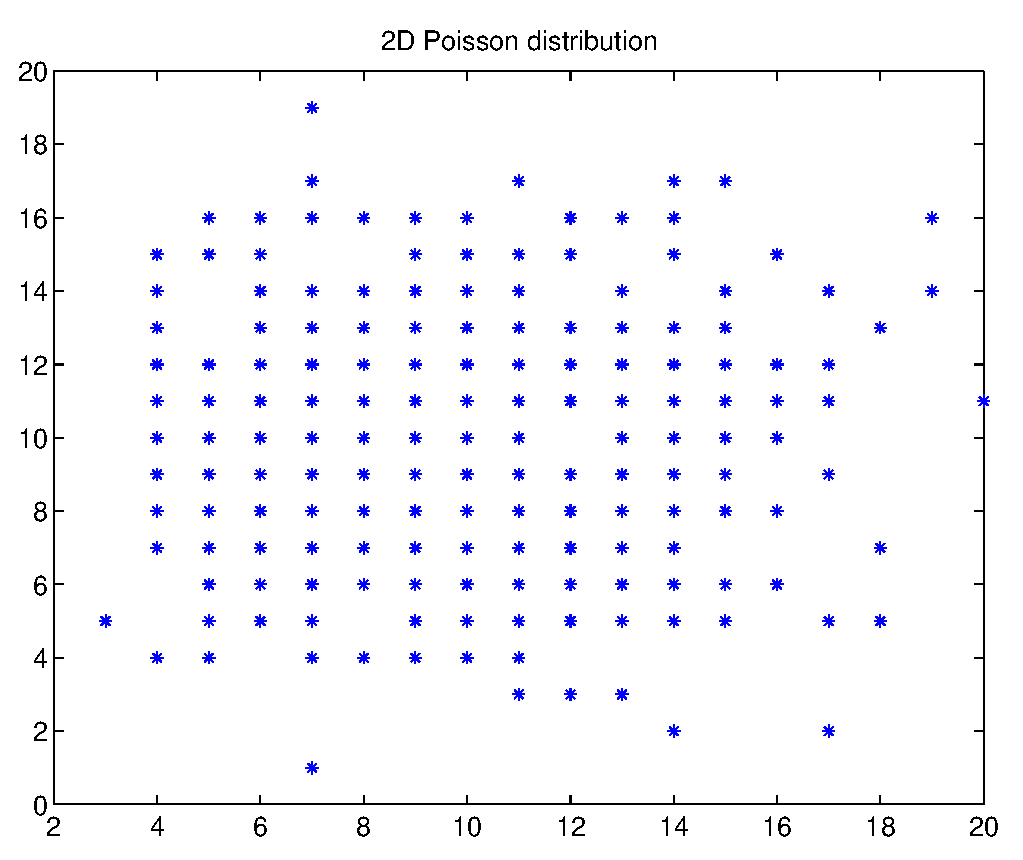
\includegraphics[width=0.47\textwidth]{f_poisson_3.eps}
  \end{center}
  \begin{center}
    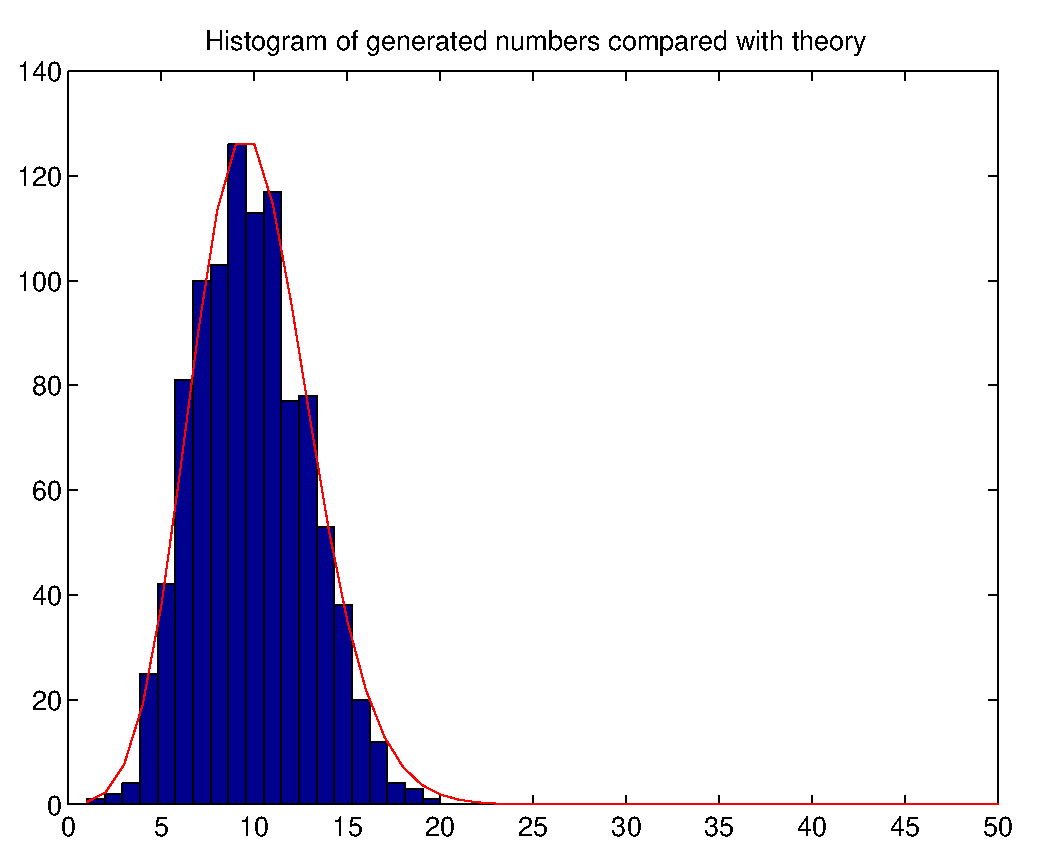
\includegraphics[width=0.8\textwidth]{f_poisson_2.eps}\hfill
  \end{center}

  Just a few comments about the method used.
  Often the Poisson distribution is written as
  $$ P_{\lambda t} (n)= e^{-\lambda t} \frac{\left(\lambda t\right)^n}{n!} ,$$
  with the parameter $\lambda t$. We have chosen $t$ to be one and so
  referring to a unit interval of time. In that sense $\lambda$ is the
  average number of events per unit time (and as you already know, it is
  actually the mean of the Poisson distribution).

  Now, the algorithm used is
  based on the fact that if the time intervals $T_i$ between events
  are from $\exp(-\lambda T_i)$, then the number of events occurring
  in an unit interval of time is from $P_\lambda(n)$ (Poisson distributed).

  To proof that, you need the theorem: if $X_1,\ldots ,X_n$ are mutually
  independent random variables with the exponential density
  $$p(x)=\lambda e^{-\lambda x}$$
  then the sum $S_N:=X_1+\cdots+X_n$ has a density
  $$ g_n(x) = \lambda \frac{(\lambda x)^{n-1}}{(n-1)!} e^{-\lambda x} .$$
  (This is a so called gamma density.) The proof can be done by
  induction. For the exponential distribution
  function $F(x)=1-e^{-\lambda x}$ we get the distribution function of $S_N$ as
  $$ G_n(x) = 1- e^{-\lambda x} \left( 1+\frac{\lambda x}{1!} + \cdots
    \frac{(\lambda x)^{n-1}}{(n-1)!} \right) .$$

  The second step is to introduce a new family of random variables
  $N(t)$: $N(t)$ is the number of indices $k\geq 1$ such that $S_k\leq t.$
  ($S_k$ is the sum opf exponentially distributed r.v. from above.)
  Because $S_n$ has the distribution $G_n(x)$ (see theorem above),
  the probability of events $\{N(t)=n\}$ has the distribution
  $$ P(\{N(t)=n\}= G_n(t)-G_{n+1}(t) = e^{-\lambda t} \frac{(\lambda t)^n}{n!}.$$
  That is exactly a Poisson distribution!

  For details see \cite[page 8-12]{feller2:71}.
\end{Solution}
\begin{Solution}{Acceptance-Rejection-Method}
\textbf{Acceptance-Rejection-Method - \texttt{rejection.m} } \\
  First of all we have to note that the volume of the n-dimensional
  sphere is given by
  $$ V_{R,n} = R^n \times V_{1,n} = R^n \times \frac{\pi^{n/2}}{\Gamma(n/2+1)},$$
  where $\Gamma(x)$ is the well known Gamma function:
  $$\Gamma(x):= \int_0^\infty e^{-t} t^{x-1} dt = \lim_{n\to\infty} n^x
    \frac{(n-1)!}{x(x+1)(x+2) \cdots (x+n-1)} \quad \text{for x >0}.$$
  (for all real numbers, except $0, -1, -2 \ldots.$
  We have $\Gamma(x+1)=x\Gamma(x)$ and therefore for natural numbers $n>0$
  $\Gamma(n+1)=n!.$ As you can see in the figure, the volume of the sphere
  (red diamonds/line)
  is decreasing by going to higher dimensions (keeping the radius $R=1$ constant).
  \begin{center}
    \hspace*{-1cm}
    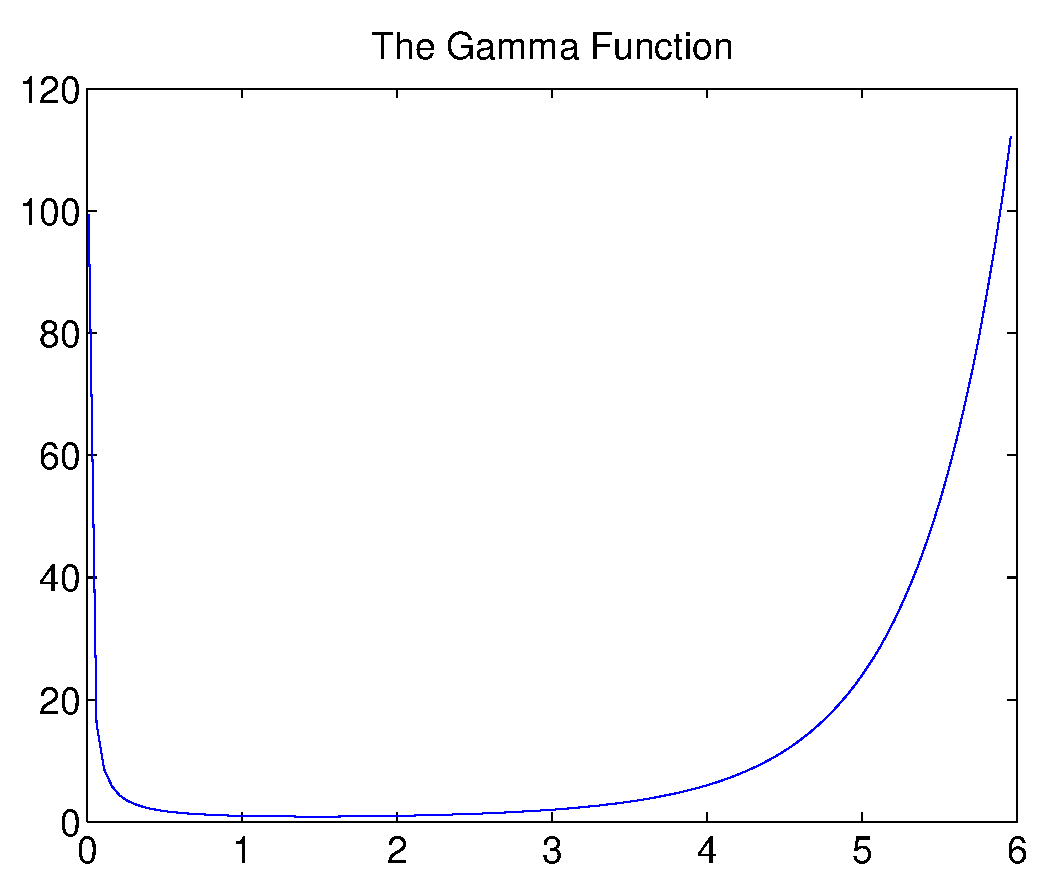
\includegraphics[width=0.47\textwidth]{f_gamma.eps}\hfill
    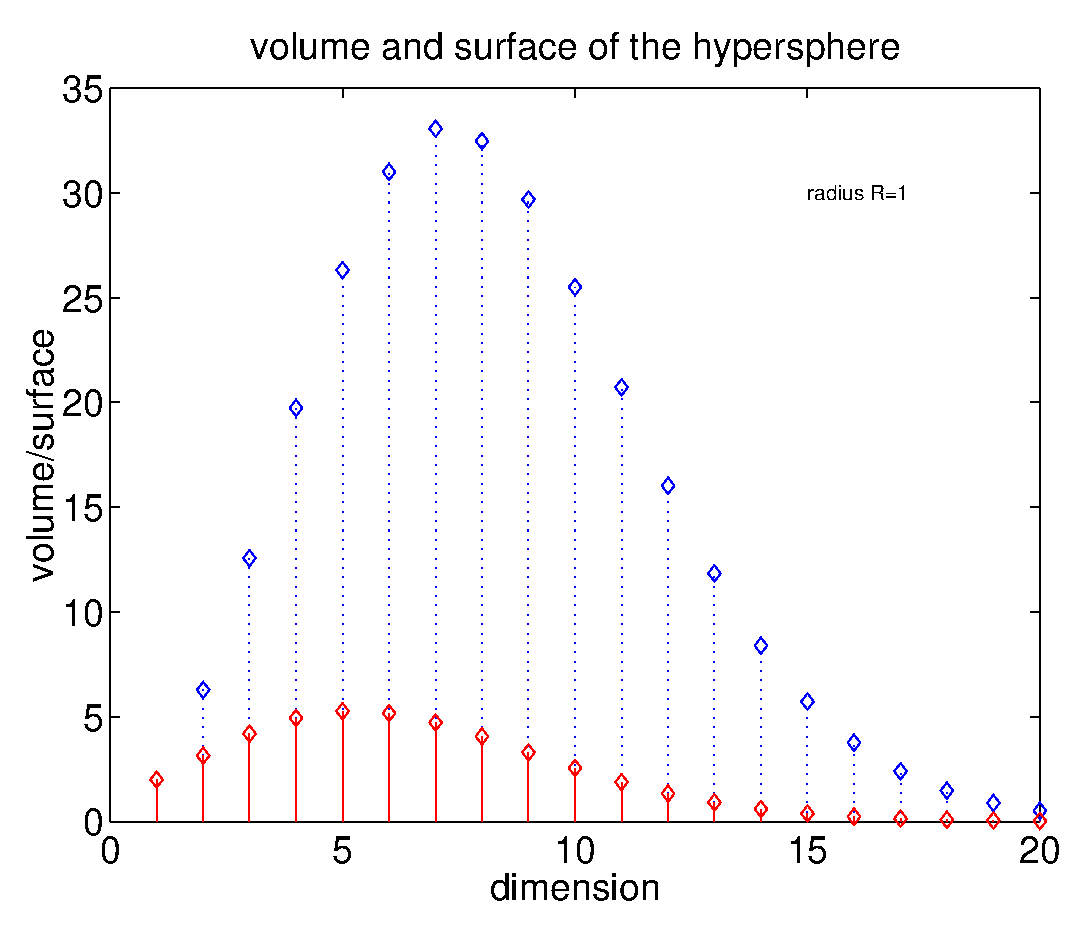
\includegraphics[width=0.47\textwidth]{f_sphere.eps}
  \end{center}

  You get the surface of the sphere by just differentiating the formula above
  and get (see blue diamonds/line)
  $$ S_{R,n} = \frac{d}{dR} V_{R,n} =
  n R^{n-1} \times \frac{\pi^{n/2}}{\Gamma(n/2+1)}.$$
  \begin{center}
    \hspace*{-1cm}
    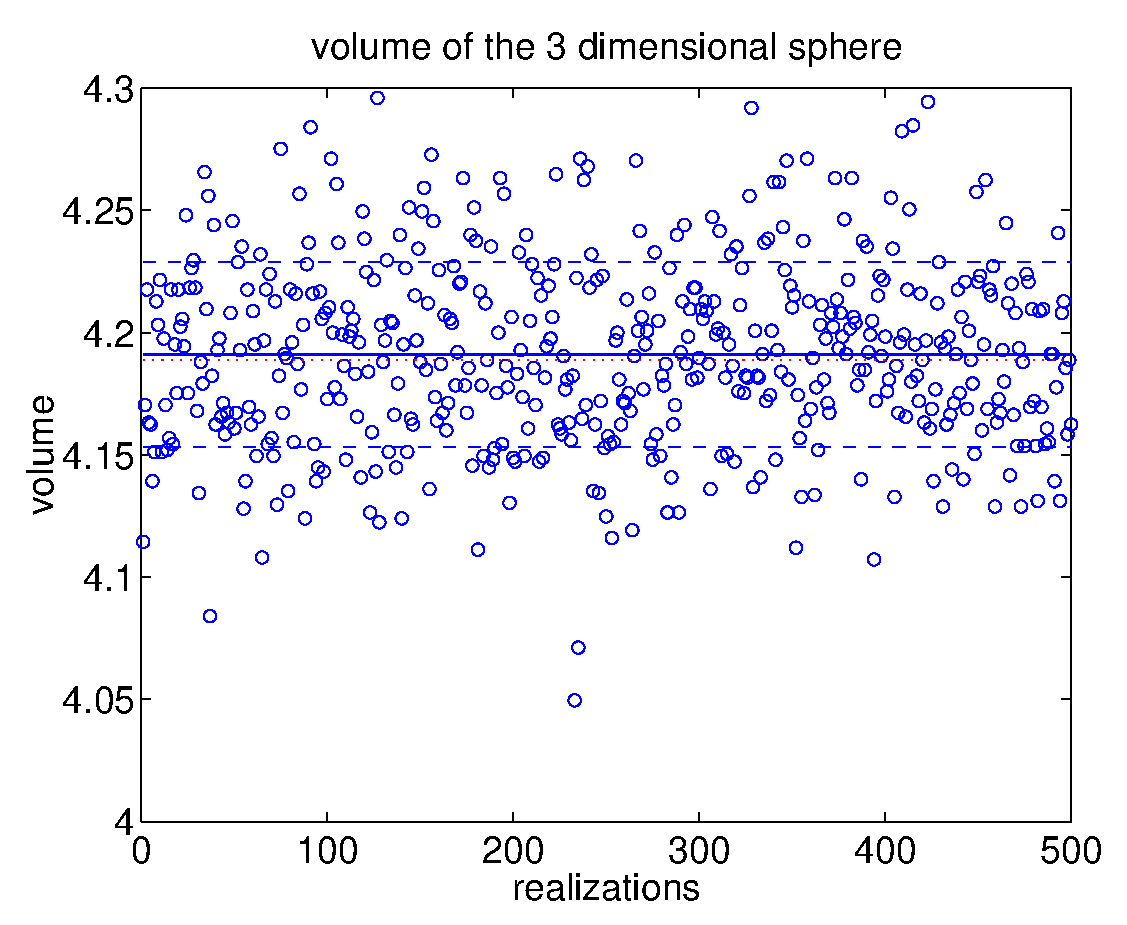
\includegraphics[width=0.47\textwidth]{f_rejection_1.eps}\hfill
    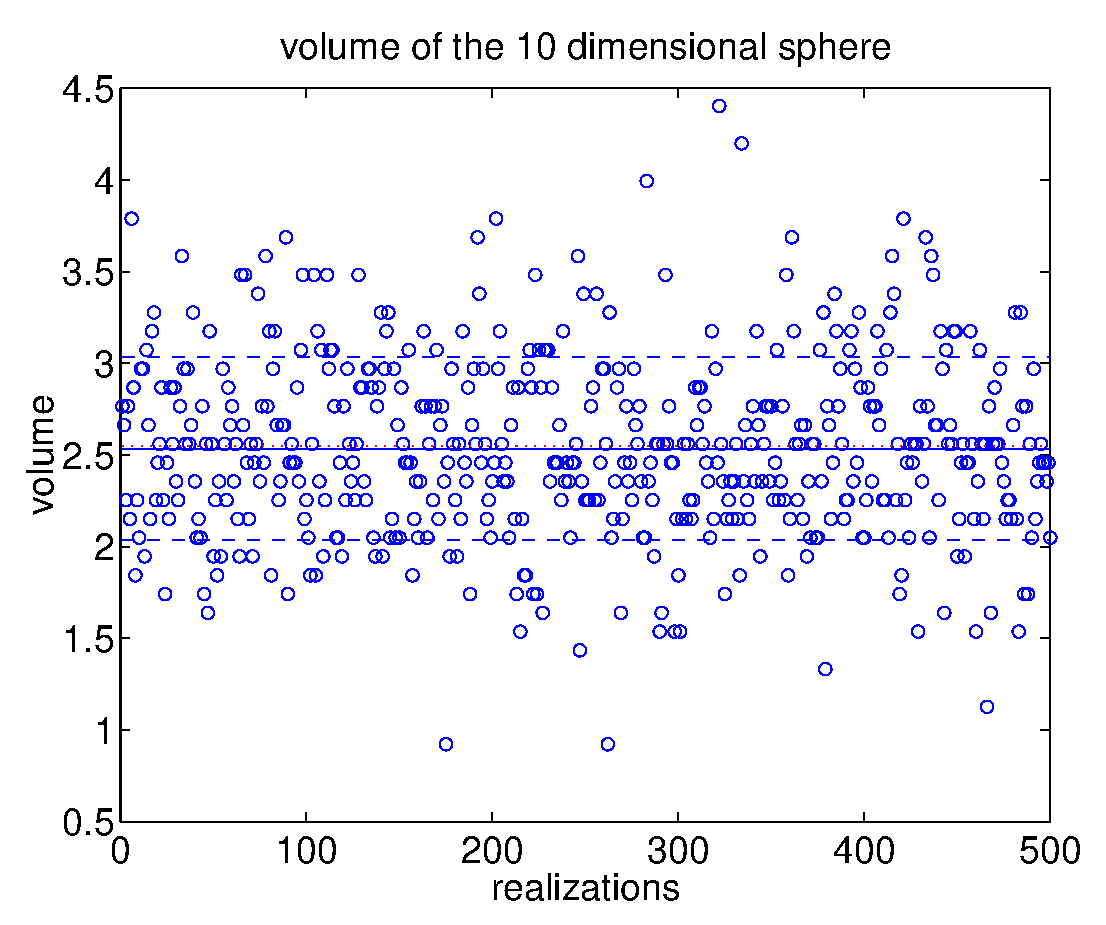
\includegraphics[width=0.47\textwidth]{f_rejection_2.eps}
  \end{center}
  The blue lines represent the sample mean and the sample variance and
  the red line is the exact value.
  Both figures are made using 500 realizations each drawing 10000 points
  in the n-dimensional space. The result for the left figure was
  $V=4,1910\pm0,0017$ (exact $V=4,1888$), for the right figure we got
  $V=2,534\pm0,022$ (exact $V=2,550$).

  The algorithm for the surface of the hyper sphere is exactly the same,
  except that in the case of an accepted hit, you have to divide the
  accepted coordinates by the radius $R$. This gives you a point on the
  surface of the sphere.
  \begin{center}
    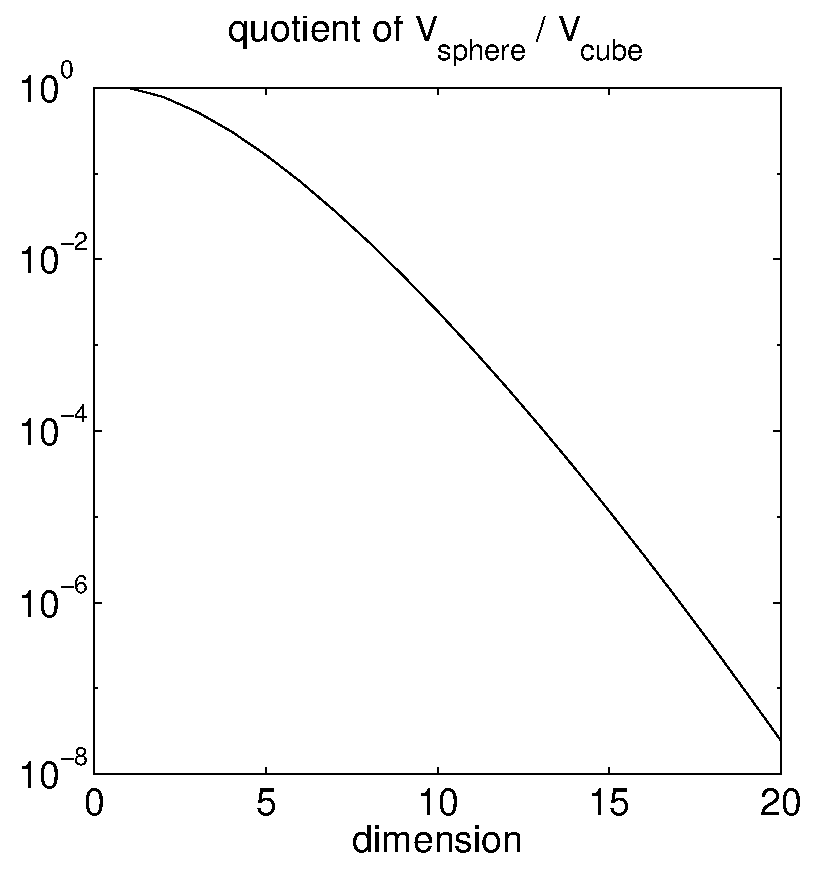
\includegraphics[width=0.47\textwidth]{f_rejection_efficiency.eps}
  \end{center}
  As you can see from the plots above, the method is getting worse with
  increasing dimension, because $V_{\text{hypersphere}}/V_{\text{hypercube}}$
  is going to zero for large $n$.
\end{Solution}

\begin{Solution}{Importance_Sampling}
\textbf{Importance Sampling - \texttt{importance.m}} \\
  The idea of the importance sampling here is instead of sampling
  uniform random numbers and putting it into the function, we
  use normally distributed random numbers.

  {\bf A very good book about importance sampling is
  \cite[Chapter 3 and 4.1]{kalos:86}.}

  \begin{itemize}
  \item Standard sampling:\\
    $$ I_S= \frac{c}{N} \sum_{i=1}^N f(\xi) ,$$
    where the $\xi$ are from a uniform distribution.\\
    Easy to implement and understand, but the error is usually very
    big.
  \item Importance sampling:\\
    Here we suggested to use a normal distribution instead of the
    uniform one for the $\xi$. Then the formula reduces to:
    $$ I_I = \frac{1}{N} \sum_{i=1}^N |\xi| \times
       \frac{\sqrt{2 \pi \sigma^2}}{2} \times \frac{1}{\sqrt{2}} =
       \frac{\sqrt{\pi}}{2 N} \sum_{i=1}^N |\xi| .$$
    First of all you have to realize that the \texttt{randn()} function
    of Matlab produces normally distr. random numbers with mean $\mu=0$
    and variance $\sigma^2=1$. It also produces random numbers in the
    open interval $(-\infty,+\infty)$ and not, like desired, in the
    interval $[0,+\infty).$

    To correct for that, use the fact, that
    $$ \int_0^\infty ve^{-v^2}dv = \frac{1}{2} \int_{-\infty}^{+\infty}
      |v| e^{-v^2}.$$
    (because the function is symmetric with respect to the y-axis.)
    Matlab produces numbers from
    $$ p(x)=\frac{1}{\sqrt{2\pi\sigma^2}}
                \exp(-\frac{(x-\mu)^2}{2\sigma^2}), \mu=0, \sigma^2=1.$$
    Now we have to transform this density to one with variance
    $\sigma^2=1/2,$ which then has the form appearing in our integral
    $(e^{-v^2}).$ We just divide the random number generated
    with \texttt{randn()} by $\sqrt{2}.$

    Then we accept only random numbers falling in the interval $[-c,c],$
    because we are integrating over that interval (we have to take this into
    account, when calulating moments). Actually we do not    
    need that restriction, but it demonstrates some additional complications, which
    could arise in actual problems.

    The last step is to correct for the additional factor
    $\sqrt{2 \pi \sigma^2}$ introduced by the normal distribution,
    and the factor $1/2$ because of the extended interval. This gives
    an overall factor of these two corrections of $\frac{\sqrt{\pi}}{2}$.
  \end{itemize}

  The first two figures show a run with 15.000 points (normally
  distributed random numbers) and a maximum cut-off $c_{\text{max}}=10.$
  That means I have done many runs with increasing $c_{\text{max}}.$
  The red boxes indicate the results of the importance sampling,
  the blue line represents the exact result.

  The figure on the right gives the systematic error involved, if
  the cut-off $c$ is used for the calculation.
  \begin{center}
    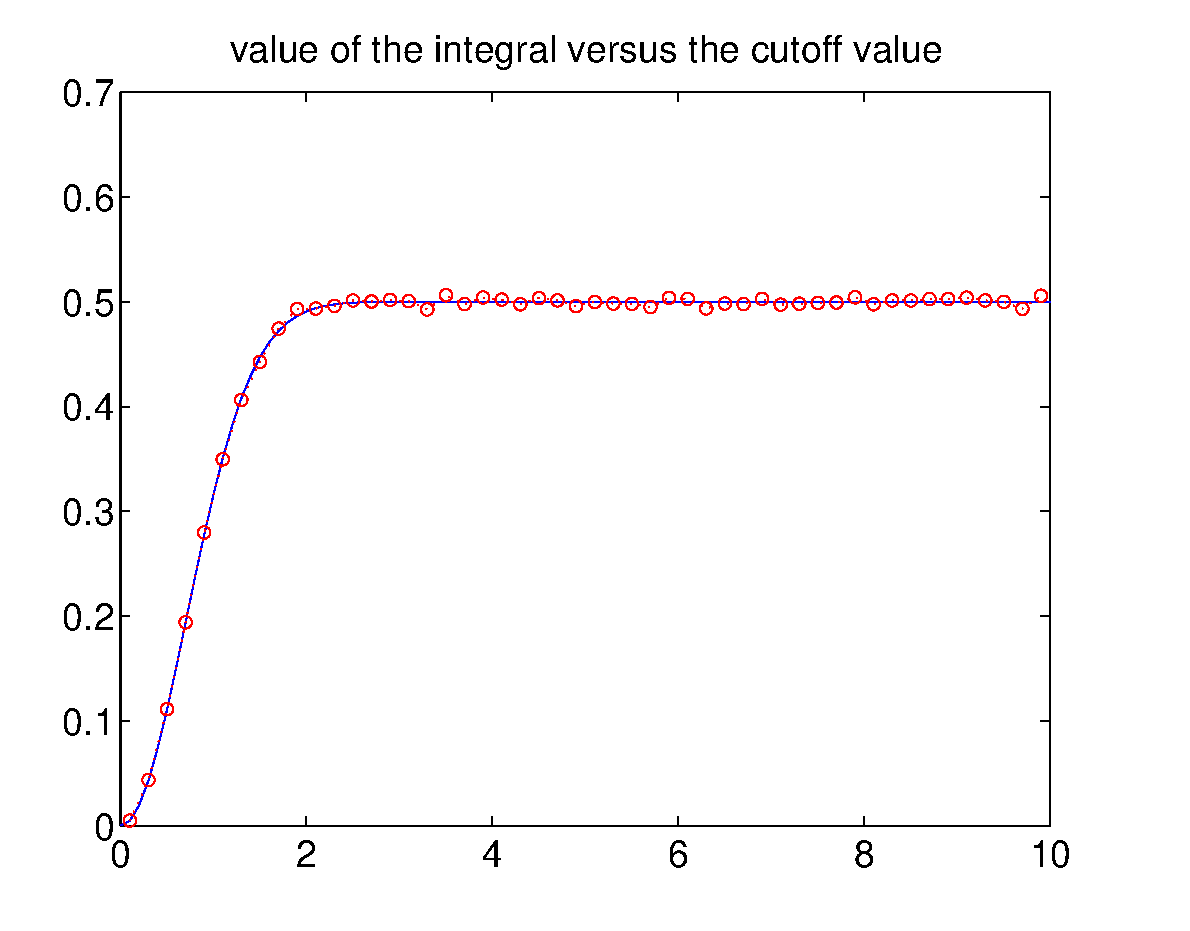
\includegraphics[width=0.47\textwidth]{f_importance_1.eps}\hfill
    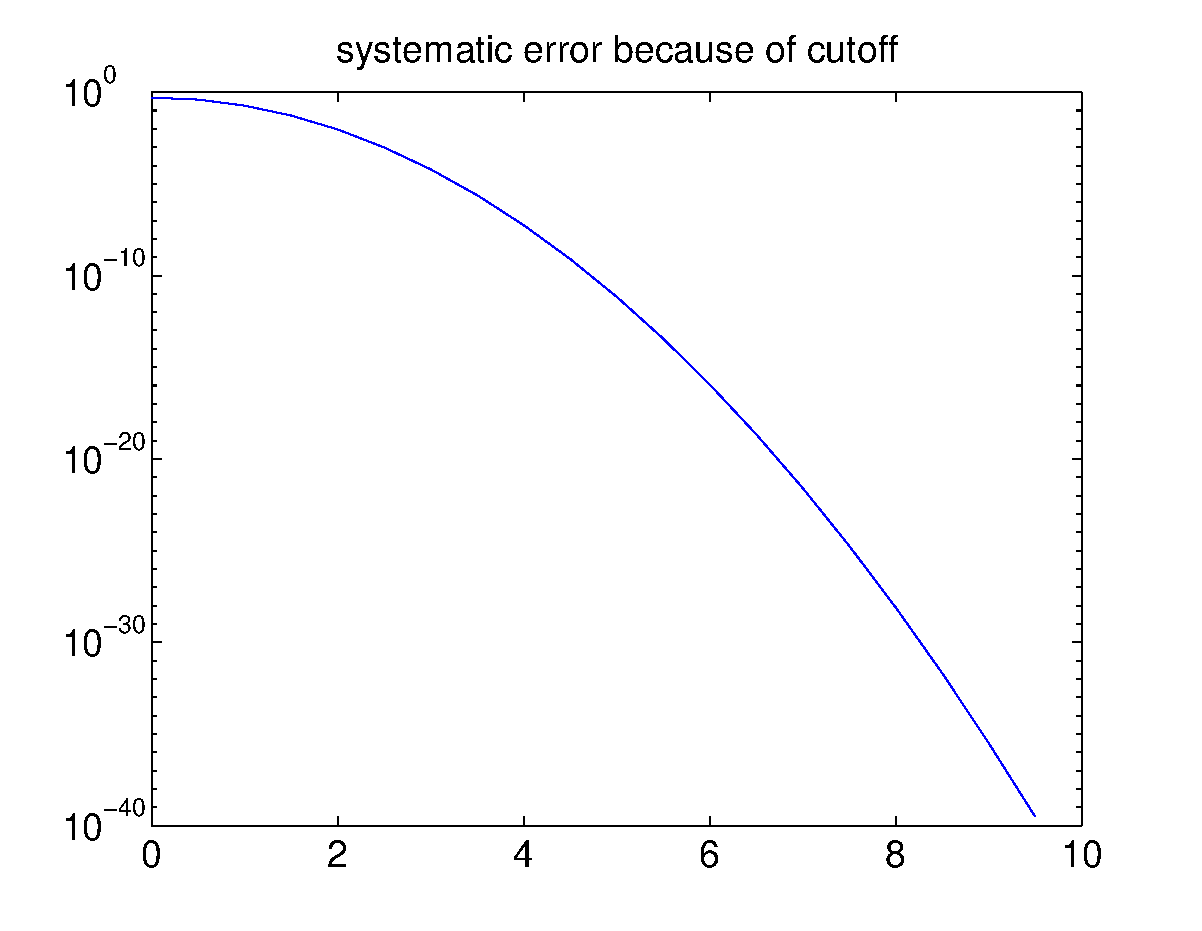
\includegraphics[width=0.47\textwidth]{f_importance_2.eps}
  \end{center}

  On the left I have plotted the function to be integrated. On the
  right there is again a result of a run using 1000 points:
  the blue line is the exact result, the red boxes are the
  importance sampling results and the black boxes are the simple
  sampling results.
  \begin{center}
    \includegraphics[width=0.47\textwidth]{f_importance_3.eps}\hfill
    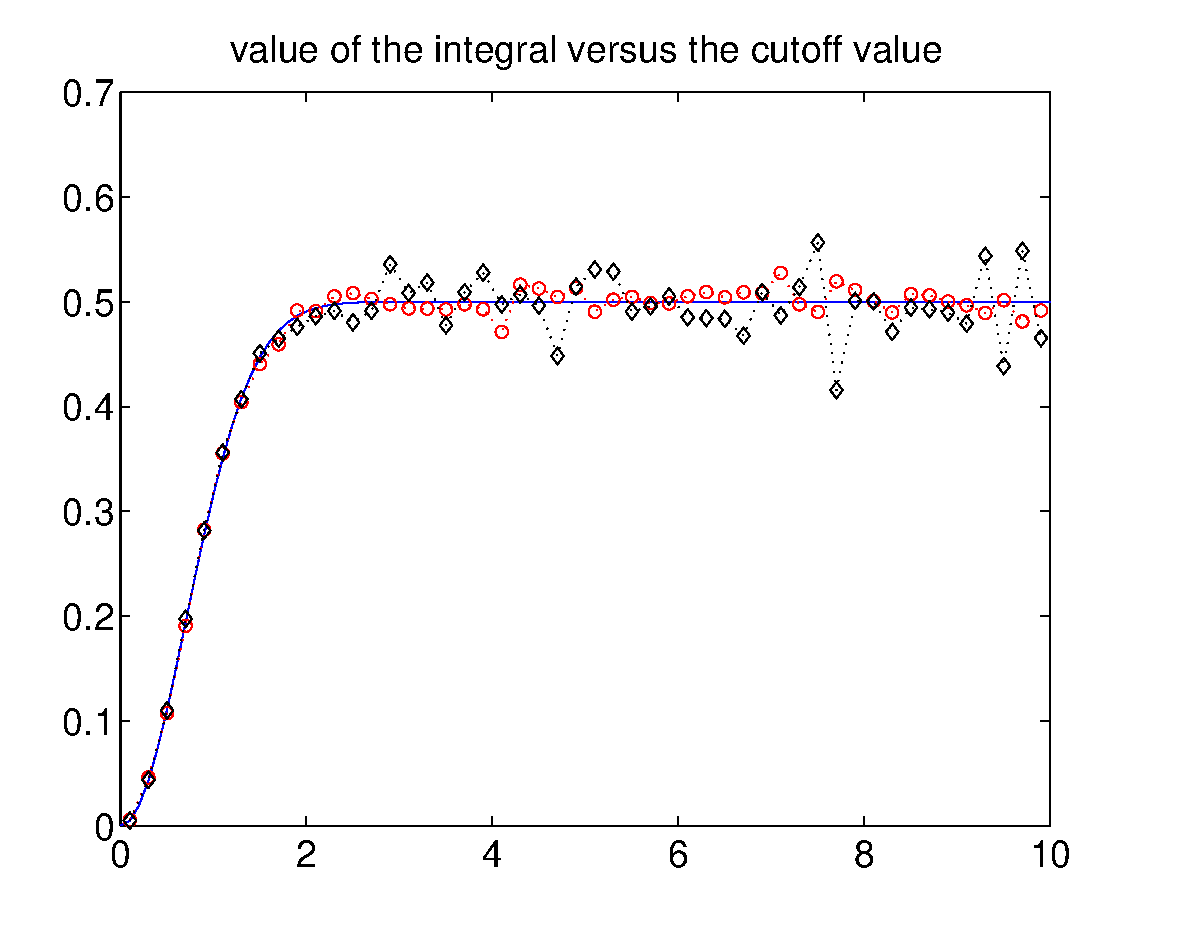
\includegraphics[width=0.47\textwidth]{f_importance_4.eps}
  \end{center}

  {\bf short discussion about (exact) variance:}\\
  The variance of the importance sampling method can be analytically
  calculated for this case. The general formula is
  $$ \sigma^2 = \int_a^b \frac{g^2(x)}{f^2(x)} f(x) dx - \overline{I}^2,$$
  where
  $$ \overline{I} = \int_a^b \frac{g(x)}{f(x)} f(x) dx $$
  is the integral we are looking for (This is just the second moment
  minus the first moment squared, as usual.).

  In our case the first moment (the solution) is just $1/2$ for the interval
  $0$ to $\infty.$ For an interval from $0$ to $c$ we have
  $$ \int_0^c v e^{-v^2} dv = 1/2-{\frac {{e^{-c^{2}}}}{2}} .$$
  The second moment is just
  $$ \int_0^c v^2 e^{-d v^2} dv = -{\frac {2\,{e^{-dc^{2}}}d^{3/2}c-
      \sqrt{\pi }{\it erf}(\sqrt {d}c)d}{4\,d^{5/2}}} .$$
  (${\it erf}(c)$ is the error function.)

  With the help of the above formulas, we can discuss three possible
  sampling functions methods: \\
  {\bf -- we use as an example $c=10$ --}
  \begin{enumerate}
  \item the standard sampling using uniform deviates $f(x)=\frac{1}{(b-a)}=1/c$:\\
    $$ \sigma^2 = \int_0^c \frac{v^2 e^{-2v^2}}{1/c^2} \frac{1}{c} dv - %
          \frac{1}{4} =  1.316642671 .$$
  \item use  importance function $f(x)= \frac{1}{\sqrt{2\pi}}
       e^{-\frac{v^2}{2}}$:\\
    $$ \sigma^2 = \int_0^c \frac{v^2 e^{-2v^2}}{1/2\pi e^{-v^2}}
       \frac{1}{\sqrt{2\pi}}e^{-\frac{v^2}{2}} dv - \frac{1}{4}
       = 0.3545997878 .$$
  \item use importance function $f(x)=e^{-v^2}$:\\
    $$ \sigma^2 = \int_0^c \frac{v^2 e^{-2v^2}}{e^{-2v^2}} e^{-v^2} dv - %
      \frac{1}{4} =  0.1931134628 .$$
  \end{enumerate}
  As you can clearly see, the variance is greatly reduced by choosing an
  importance function very close to the function to be integrated.
  And of course the simple sampling Monte Carlo integration produces a
  big variance compared to the importance sampling method (here almost
  a factor of $4$ to $6$.).
\end{Solution}

\begin{Solution}{First_Passage_Times}
\textbf{First Passage Times (fpt) - \texttt{first\_passage.m}} \\
  The left figure shows a run using $R=5$ and 10.000 walks. The mean
  first passage time is $30,03$ steps.

  On the right, I have done many runs with different $R$ and calculated
  the mean first passage time for each run. You can see the exponential
  growth of the mean fpt.

  \begin{center}
    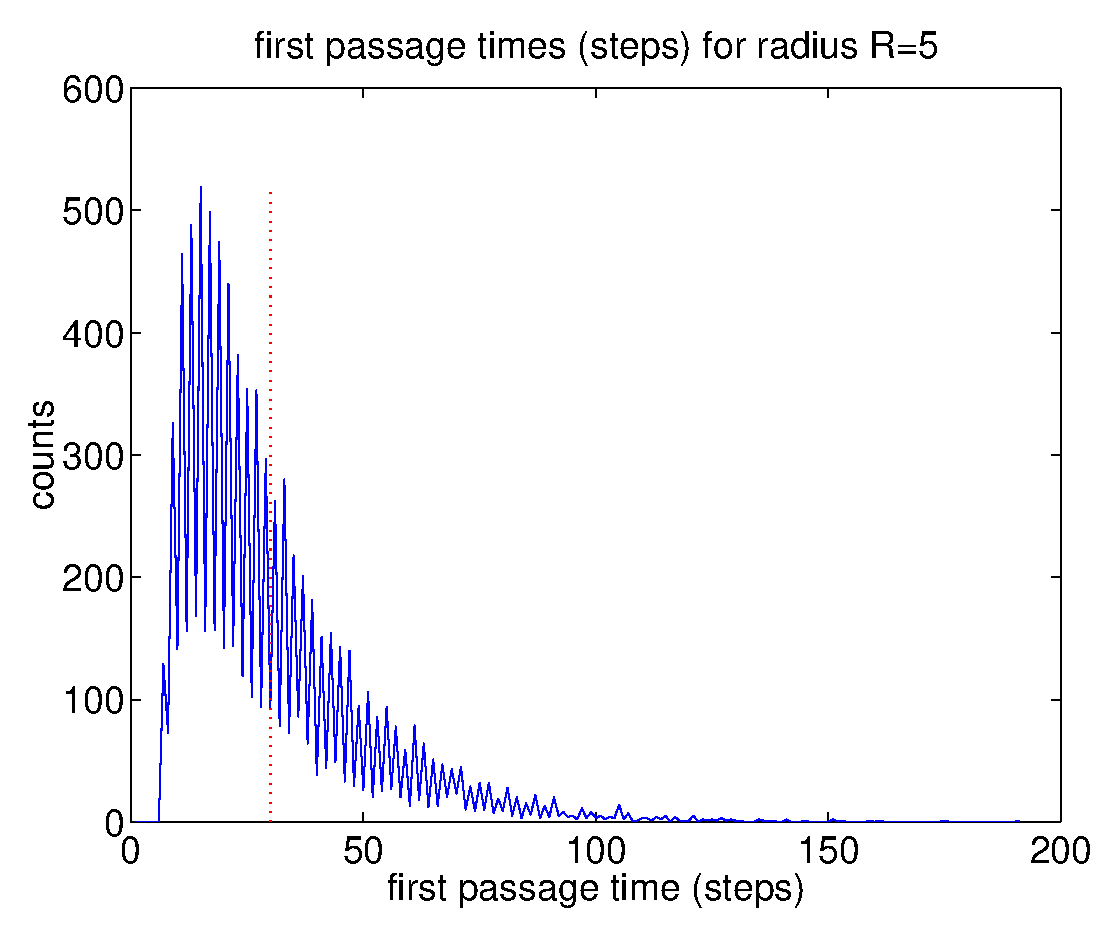
\includegraphics[width=0.47\textwidth]{f_firstpassage_1.eps}\hfill
    \includegraphics[width=0.47\textwidth]{f_firstpassage_2.eps}
  \end{center}
\end{Solution}

%%%%%%%%%%%%%%%%%%%%%%%%%%%%%%%%%%%%%%%%%%%%%%%%%%%%%%%%%%%%%%%
\section{Solutions to Chapter 4}

\begin{Solution}{}
\end{Solution}

\begin{Solution}{}
\end{Solution}

%%%%%%%%%%%%%%%%%%%%%%%%%%%%%%%%%%%%%%%%%%%%%%%%%%%%%%%%%%%%%%%
\section{Solutions to Chapter 5}
\begin{Solution}{}
\end{Solution}
%%%%%%%%%%%%%%%%%%%%%%%%%%%%%%%%%%%%%%%%%%%%%%%%%%%%%%%%%%%%%%%
\section{Solutions to Chapter 6}
\begin{Solution}{}
\end{Solution}
%%%%%%%%%%%%%%%%%%%%%%%%%%%%%%%%%%%%%%%%%%%%%%%%%%%%%%%%%%%%%%%
\section{Solutions to Chapter 7}

%%%%%%%%%%%%%%%%%%%%%%%%%%%%%%%%%%%%%%%%%%%%%%%%%%%%

\bibliographystyle{peter}
\bibliography{V_98,simulit}


%%%%%%%%%%%%%%%%%%%%%%%%%%%%%%%%%%%%%%%%%%%%%%%%%%%%
